\documentclass[11pt,a4paper]{article}

% French
\usepackage[utf8x]{inputenc}
\usepackage[frenchb]{babel}
\usepackage[T1]{fontenc}
\usepackage{lmodern}
\usepackage{ifthen}

% Color
% cfr http://en.wikibooks.org/wiki/LaTeX/Colors
\usepackage{color}
\usepackage[usenames,dvipsnames,svgnames,table]{xcolor}
\definecolor{dkgreen}{rgb}{0.25,0.7,0.35}
\definecolor{dkred}{rgb}{0.7,0,0}

% Floats and referencing
\newcommand{\sectionref}[1]{section~\ref{sec:#1}}
\newcommand{\annexeref}[1]{annexe~\ref{ann:#1}}
\newcommand{\figuref}[1]{figure~\ref{fig:#1}}
\newcommand{\tabref}[1]{table~\ref{tab:#1}}
\usepackage{xparse}
\NewDocumentEnvironment{myfig}{mm}
{\begin{figure}[!ht]\centering}
{\caption{#2}\label{fig:#1}\end{figure}}

% Listing
\usepackage{listings}
\lstset{
  numbers=left,
  numberstyle=\tiny\color{gray},
  basicstyle=\rm\small\ttfamily,
  keywordstyle=\bfseries\color{dkred},
  frame=single,
  commentstyle=\color{gray}=small,
  stringstyle=\color{dkgreen},
  %backgroundcolor=\color{gray!10},
  %tabsize=2,
  rulecolor=\color{black!30},
  %title=\lstname,
  breaklines=true,
  framextopmargin=2pt,
  framexbottommargin=2pt,
  extendedchars=true,
  inputencoding=utf8x
}

\newcommand{\matlab}{\textsc{Matlab}}
\newcommand{\octave}{\textsc{GNU/Octave}}
\newcommand{\qtoctave}{\textsc{QtOctave}}
\newcommand{\oz}{\textsc{Oz}}
\newcommand{\java}{\textsc{Java}}
\newcommand{\clang}{\textsc{C}}
\newcommand{\keyword}{mot clef}

% Math symbols
\usepackage{amsmath}
\usepackage{amssymb}
\usepackage{amsthm}
\DeclareMathOperator*{\argmin}{arg\,min}
\DeclareMathOperator*{\argmax}{arg\,max}

% Sets
\newcommand{\Z}{\mathbb{Z}}
\newcommand{\R}{\mathbb{R}}
\newcommand{\Rn}{\R^n}
\newcommand{\Rnn}{\R^{n \times n}}
\newcommand{\C}{\mathbb{C}}
\newcommand{\K}{\mathbb{K}}
\newcommand{\Kn}{\K^n}
\newcommand{\Knn}{\K^{n \times n}}

% Chemistry
\newcommand{\std}{\ensuremath{^{\circ}}}
\newcommand\ph{\ensuremath{\mathrm{pH}}}

% Theorem and definitions
\theoremstyle{definition}
\newtheorem{mydef}{Définition}
\newtheorem{mynota}[mydef]{Notation}
\newtheorem{myprop}[mydef]{Propriétés}
\newtheorem{myrem}[mydef]{Remarque}
\newtheorem{myform}[mydef]{Formules}
\newtheorem{mycorr}[mydef]{Corrolaire}
\newtheorem{mytheo}[mydef]{Théorème}
\newtheorem{mylem}[mydef]{Lemme}
\newtheorem{myexem}[mydef]{Exemple}
\newtheorem{myineg}[mydef]{Inégalité}

% Unit vectors
\usepackage{esint}
\usepackage{esvect}
\newcommand{\kmath}{k}
\newcommand{\xunit}{\hat{\imath}}
\newcommand{\yunit}{\hat{\jmath}}
\newcommand{\zunit}{\hat{\kmath}}

% rot & div & grad & lap
\DeclareMathOperator{\newdiv}{div}
\newcommand{\divn}[1]{\nabla \cdot #1}
\newcommand{\rotn}[1]{\nabla \times #1}
\newcommand{\grad}[1]{\nabla #1}
\newcommand{\gradn}[1]{\nabla #1}
\newcommand{\lap}[1]{\nabla^2 #1}


% Elec
\newcommand{\B}{\vec B}
\newcommand{\E}{\vec E}
\newcommand{\EMF}{\mathcal{E}}
\newcommand{\perm}{\varepsilon} % permittivity

\newcommand{\bigoh}{\mathcal{O}}
\newcommand\eqdef{\triangleq}

\DeclareMathOperator{\newdiff}{d} % use \dif instead
\newcommand{\dif}{\newdiff\!}
\newcommand{\fpart}[2]{\frac{\partial #1}{\partial #2}}
\newcommand{\ffpart}[2]{\frac{\partial^2 #1}{\partial #2^2}}
\newcommand{\fdpart}[3]{\frac{\partial^2 #1}{\partial #2\partial #3}}
\newcommand{\fdif}[2]{\frac{\dif #1}{\dif #2}}
\newcommand{\ffdif}[2]{\frac{\dif^2 #1}{\dif #2^2}}
\newcommand{\constant}{\ensuremath{\mathrm{cst}}}

% Numbers and units
\usepackage[squaren, Gray]{SIunits}
\usepackage{sistyle}
\usepackage[autolanguage]{numprint}
%\usepackage{numprint}
\newcommand\si[2]{\numprint[#2]{#1}}
\newcommand\np[1]{\numprint{#1}}

\newcommand\strong[1]{\textbf{#1}}
\newcommand{\annexe}{\part{Annexes}\appendix}

% Bibliography
\newcommand{\biblio}{\bibliographystyle{plain}\bibliography{biblio}}

\usepackage{fullpage}
% le `[e ]' rend le premier argument (#1) optionnel
% avec comme valeur par défaut `e `
\newcommand{\hypertitle}[7][e ]{
\usepackage{hyperref}
{\renewcommand{\and}{\unskip, }
\hypersetup{pdfauthor={#6},
            pdftitle={Synth\`ese d#1#2 Q#3 - L#4#5},
            pdfsubject={#2}}
}

\title{Synth\`ese d#1#2 Q#3 - L#4#5}
\author{#6}

\begin{document}

\ifthenelse{\isundefined{\skiptitlepage}}{
\begin{titlepage}
\maketitle

 \paragraph{Informations importantes}
   Ce document est grandement inspiré de l'excellent cours
   donné par #7 à l'EPL (École Polytechnique de Louvain),
   faculté de l'UCL (Université Catholique de Louvain).
   Il est écrit par les auteurs susnommés avec l'aide de tous
   les autres étudiants, la vôtre est donc la bienvenue.
   Il y a toujours moyen de l'améliorer, surtout si le cours
   change car la synthèse doit alors être modifiée en conséquence.
   On peut retrouver le code source à l'adresse suivante
   \begin{center}
     \url{https://github.com/Gp2mv3/Syntheses}.
   \end{center}
   On y trouve aussi le contenu du \texttt{README} qui contient de plus
   amples informations, vous êtes invité à le lire.

   Il y est indiqué que les questions, signalements d'erreurs,
   suggestions d'améliorations ou quelque discussion que ce soit
   relative au projet
   sont à spécifier de préférence à l'adresse suivante
   \begin{center}
     \url{https://github.com/Gp2mv3/Syntheses/issues}.
   \end{center}
   Ça permet à tout le monde de les voir, les commenter et agir
   en conséquence.
   Vous êtes d'ailleurs invité à participer aux discussions.

   Vous trouverez aussi des informations dans le wiki
   \begin{center}
     \url{https://github.com/Gp2mv3/Syntheses/wiki}.
   \end{center}
   comme le statut des synthèses pour chaque cours
   \begin{center}
     \url{https://github.com/Gp2mv3/Syntheses/wiki/Status}.
   \end{center}
   vous pouvez d'ailleurs remarquer qu'il en manque encore beaucoup,
   votre aide est la bienvenue.

   Pour contribuer au bug tracker et au wiki, il vous suffira de
   créer un compte sur Github.
   Pour interagir avec le code des synthèses,
   il vous faudra installer \LaTeX.
   Pour interagir directement avec le code sur Github,
   vous devez utiliser \texttt{git}.
   Si cela pose problème,
   nous sommes évidemment ouverts à des contributeurs envoyant leurs
   changements par mail ou n'importe quel autre moyen.
\end{titlepage}
}{}

\ifthenelse{\isundefined{\skiptableofcontents}}{
\tableofcontents
}{}
}


\hypertitle{en}{Artificial Intelligence}{7}{INGI}{2261}
{Nicolas Houtain\and Symeon Malengreau\and Gorby Nicolas Ndonda Kabasele}
{Yves Deville}

\textbf{ATTENTION: We should complete the content of this chapter with the content of the book}

\section{Chapitre 1 : Introduction}

\textbf{What is IA ?}
\begin{itemize}
\item System that think like human
\item System that act like human
\item System that think like rationnally
\item System that act rationnally
\end{itemize}
Think is the process which lead to do an action while act is the behaviour, the action. 
\subsection{Turing test approach}
A \textbf{AI} succcess if it make a human think that he's speaking with a human.
\section{Chapitre 2.1-2.3, Intelligent Agent}

\subsection{Agents and environments}
\begin{description}

    \item[Agent]  :  Anything  that  can be  viewed  as  perceiving  its
    environment through sensor and acting through actuators.

    \item[Percept] : Refer to the agent's perceptual inputs at any given
        instant

    \item[Percept sequence] : Complet history of percept

\end{description}

\subsection{Concept of rationality}
\begin{description}

    \item[Rationality] : Is do the right think, but what is the
        right think for computer? Need \textit{Performance measure}

    \item[Rationnal  agent]  : For  each  possible  percept sequence,  a
    rational agent should select an  action that is expected to maximize
    its performance measure, given the  evidence provided by its percept
    sequence and whatever build-in knowledge the agent has.
    

   \item What is rationnal all the time is:
        \begin{enumerate}
            \item Performance measure that define the criterion of success
            \item Knowledge of the environment by the agent
            \item Action that the agent can perform
            \item Percept sequence up to date
        \end{enumerate}
	
    \item The performance of an agent is measurde by the sequence of action that it does. If the sequence is
    		desirable, then it performs well.
    \item Note : Rationnality $\neq$ omniscience, (expected performance $\neq$ actual performance)

    \item[Omniscience agent] : know the \textbf{real} result of its action.

    \item[Autonomy] :  An automous agent learn what it can do to compensate for partial or incorrect prior
    knowledge. (It shouldn't only rely on its prior knowledge)

\end{description}


\subsection{Nature of environments}
Task environnement (PEAS) is a specification to the \textbf{P}erformance, 
\textbf{E}environment, \textbf{A}ctuators ans \textbf{S}ensors.

\begin{figure}[h]
    \centering
    \begin{tabular}{|m{3cm}|m{3cm}|m{3cm}|m{3cm}|}
        \hline
        Perf measure & Environment & Actuators & Sensors \\
        \hline
        Safe, fast, legal, max profit  & Roard, other traffic, customer,
        pedestrians &  Accelerator, display,  brake, signal  & Camerass,
        sonar, speedometer, FPS,\ldots \\
        \hline

    \end{tabular}
    \caption{Example PEAS for taxi driver}
\end{figure}
The properties of the enviromnent are the following:
\begin{description}
\item[Fully observable vs Partially observable :] All relevant information are accessible (chess vs poker)
\item[Single agent vs Multiagent:] Are there more than one agent, if yes then it can a cooperation or a 
competition. (crossword puzzle vs chess)
\item[Deterministic vs Stochastic:] The next state of the enviromnent depends entirely on the action of the 
agent. (chess vs poker)
\item[Episodic vs Sequential:] Experience of the agent is divided into atomic episode that are independent 
from each other.
\item[Static vs Dynamic:] The enviromnent can change while the agent is thinking. If the performance of the 
agent change over the course of time, then its \textbf{Semidynamic}.(crossword vs chess with clock)
\item[Discrete vs Continuous:] The number of distinct state is finite and the sets of action and percepts are 
discrete. (chess vs taxi driving)
\item[Known vs Unknown:]  The outcome for all action are given. Not the same as fully observable,for 
example video game, know all the information via the screen but dont' know what the button does.

\end{description}

\subsection{Structure of Agent}
An agent is composed of two parts:
\begin{itemize}
\item The \textbf{architecture} which is the computer device on which the agent is running.
\item The \textbf{program} which is a function that map the percepts to the action. 
\end{itemize}
In genral, the architecture makes ther percepts from the \textbf{sensors} available to the program, runs the 
program, and feeds the program's action choices to the actuators as they are generated.

There exists different kind of agent:
\begin{description}
\item[Table-driven] a table of percept and a function that maps an action to the percept.
\item[Simple reflex] agent that act depending on the current percept. Based on a condition-action 
rule.
\item[Model-based reflex agent] keeps a internal representation of the enviromnent.
\item[Goal-based] same as model-based except that the agent keeps a set of goal state.
\item[Utility-based] use a utility function to choose between state.
\item[Learning] update it's behaviour by experience. It should be able to know how it performs. 
\end{description}
\section{Chapitre 3 : Solving problems by searching}

\subsection{Key principles}

\begin{description}
    \item[Search] process of looking for a (or the best) sequence of actions, that leads to a goal (specific state of the environment), starting from an initial state
    \item[States] distinguishables stages during the problem solving process (representation of physical configuration)
    \item[State space] is graph representation of the successor function with the cost.
    \item[Initial state] The state that the agent start in.
    \item[Action] an action transports the agent from one state to another one by applying an \textit{operator} 
    to a state
    \item[Transition model] A function that returns the state that results from doing action a in state s
    \item[Successor] Any state reachable from a given state
    \item[Path] Sequence of state connected by a sequence of action.
    \item[Operators] \textit{to complete}
    \item[Goal test] A test that specify if a given state is a goal state.
    \item[Step cost] numeric cost of taking action a in state s to get to s'.
    \item[Path cost] A function that assigned a numeric cost to each path.
    \item[Solution] a solution is a sequence of actions leading from the initial state to a goal state.
    \item[Optimal solution] an optimal solution has the lowest path cost among all solutions
    \item[Node] data structure constituting part of a search tree/graph and representing a state.
    \item[Frontier] set of generated nodes, which ancestors have been goal-tested (visited)
\end{description}

\subsection{Problem solving agents}

\textit{An  agent with  several immediate  options of  unknown value  can
decide what to do by first  exmining future actions that eventually lead
to states of known value}

\paragraph{Assumption} : Environment is  static, deterministic and fully
observable.

\subsubsection{Problem definition}
A problem can be defined :
\begin{enumerate}
    \item States and \textbf{initial state}
    \item A description of the  \textbf{possible action} available to the
    agent. 
    \item A description of what each action does, called \textbf{transition
        model}. 
    \item A \textbf{Goal test}
    \item A \textbf{Path cost} that use a step cost.
\end{enumerate}

\subsubsection{Solution} 
A  \textbf{solution}  is a  sequence  of actions  leading
from  the  initial state  to  a  goal state  A  \textcolor{red}{optimal}
\textbf{solution} has the lowest path cost amoung all solutions.

\subsubsection{State space}
Together,   initial  state,   actions   and   transition  model   define
\textbf{state space}  of the  problem. (\textit{Graph  representation of
the successor function with the cost})

\subsubsection{Abstraction}
Removing detail from a representation of the state or the action.

\subsection{Example}
For eight puzzle
\begin{itemize}
\item The state is the position of all the 8 tiles and the empty one.
\item The initial state is a random, any state can be the initial one.
\item The action are simply moving the blank space in four direction, up, down, left and right.
\item The tr	ansition model returns the effect of moving the blank space in one of the four direction.
\item The goal test is to check if the state is in the wanted configuration. (tiles in order)
\item The step is one, so the path cost is the number of step done in the path.
\end{itemize}

\subsection{Searching for Solutions}

\begin{description}

    \item[Searching] for solutions  is a traversal of  some search space
    from the \textit{initial  state} to the \textit{goal  state} using a
    legal sequence of actions (as defined by operators).

    \item[Expanding]  :  apply  each   legal  action  to  current  state
    (=generating state)

    \item[Frontier] : set of all leaf nodes available for expansion. 
        (That correspond of all leaf nodes wich ancestor have visited)
\end{description}

\paragraph{Loopy path} A  complete search tree can be  infinite if there
is  looping. But  we  don't considere  this one  because  path cost  are
additive and  steo cost are  nonnegative. (\textit{Loppy path  is nerver
better than same path without loop})

\subparagraph{ } To avoid redundant path, we use \textbf{graph search}
by using \textit{explored set}

\subsubsection{Tree and Graph Search}

There is two way to  perform the search\footnote{the slides specifies an
algorithm to search in a tree}.

\begin{itemize}

    \item \textbf{A  graph representing the state  space}: you represent
all the possible states as a graph, and you move between those states

    \item \textbf{A  search tree}: you  list all the  possibilities from
the current states using the possible \textit{operators}

\end{itemize}

\subsubsection{States and Node}
\begin{itemize}
    \item A \textbf{state} is a representation of a physical
        configuration
    \item A \textbf{node} is a data structure contituting part
        of a search tree
\end{itemize}

So, there can be many node with same state!

\subsubsection{Repeated States}

Failure  to detect  repeated states  can turn  a solvable  problems into
unsolvable ones. We are going to  avoid visiting nodes that have already
been visited.

Use \textbf{graph  search} is like tree  search but do not  expand nodes
with a state appearing in some already visited node


\subsubsection{Algorithm description}
For the tree search
	\begin{enumerate}
	\item Initialize the frontier with the initial state
	\item Loop
		\begin{enumerate}
			\item If the frontier is empty then return failure
			\item Choose a state in the frontier
			\item Check if goal test (if yes return solution path), if not expand it and add resulting state in the
			frontier
		\end{enumerate}
\end{enumerate}
For the graph is the same except that it keep an exploring set (contains the node visited) and does not 
expand the the node if it's in the exploring set.
\subsubsection{Search strategies}

There is two types of  search: \textbf{uninformed search} where the only
information known  by the agent  is \textit{Am I  on the goal?}  and the
\textbf{informed search} where agent  has a background information about
the problem.

We can evaluate a search strategy with 4 criterias:
\begin{itemize}
    \item \textbf{Completeness}: it finds a solution if one exists
    \item \textbf{Time complexity}: usually in terms of the number of nodes generated/expanded
    \item \textbf{Space complexity}: maximum nodes in memory
    \item \textbf{Optimality}: it finds a least cost solution?
\end{itemize}
And you use 3 differents variables:
\begin{itemize}
    \item $\textbf b$  maximum branching factor of the search tree (the maximum number of subnodes)
    \item $\textbf d$  depth (in the tree) of the least-cost solution
    \item $\textbf m$  maximum depth of he search tree (may be infinite)
\end{itemize}



\subsection{Uninformed search}
Here will be presented different algorithm to search in a tree.

\begin{figure}[h]
\centering
\begin{tabular}{|l|m{2cm}|m{2cm}|m{2cm}|m{2cm}|m{2cm}|m{2cm}|}
\hline
& \textbf{BFS} & \textbf{UCS} & \textbf{DFS} & \textbf{DLS} & \textbf{IDS} & \textbf {BDS}\\
\hline
& level by level & cheap path & last depth & limited depth & iterative depth & bi direct  \\

\hline
\hline
\textbf{Complete} & \textcolor{red}{if} \textbf{b} finite & \textcolor{red}{if} \textbf{sp} > 0  & NO  & \textcolor{red}{if} $l\geq d$ & YES & YES\\
\hline
\textbf{Optimale} & \textcolor{red}{if} \textbf{sp} = 1 & YES & NO & \textcolor{red}{if} l==d & \textcolor{red}{if} += 1 & \textcolor{red}{if} \textbf{sp} = 1 \\
\hline
\textbf{Time} & $b^{d+1}$    & $b^{1 + C/\epsilon}$ & $b^m$ & $b^l$ & $b^d$ & $b^{d/2}$\\
\hline
\textbf{Space} & $b^{d+1}$ & $b^{1 + C/\epsilon}$ & $bm$ & $bl$ & $bd$ & $b^{d/2}$ \\
\hline
Frontier & FIFO & Priority & LIFO & LIFO & LIFO & FIFO \\
\hline

\end{tabular}
\caption{Uninformed Search Algorithm}
\end{figure}


\subsubsection{Algorithm: Breadth-First Search}
The goal is to search in a tree level by level from "left" to "right".

The memory use grow really fast! 

You start from the root node and adds the subnodes at the end of a 
\textcolor{red}{FIFO queue} (the queue beeing the \textit{frontier}). 

\paragraph{Criteria} \textit{Complete} if b is finite and \textit{optimal} if the cost per
step is 1 (but in general use it ain't \textit{optimal}).

\paragraph{Complexity} \textit{Time complexity} of $O(b^d)$\footnote{Time complexity: $1+b+b^2+...+b^d+b(b^d-1) = O(b^{d+2}) = O(b^d)$} and a \textit{space complexity} of $O(b^d)$. 

\subsubsection{Algorithm: Uniform-Cost search}

Like a BFS but this is not the shortest path but the \textbf{cheapest} path.

This is similar to Breadth-First but with a cost adedd the the reachable
nodes. The frontier is handled as a priority queue where the node with the minimum step cost is expanded first.

The \textit{path  cost} is simply the sum of  the individual edge
costs  to reache  the current  node.  \textit{Frontier} is  now a  queue
ordered by the path cost.

\paragraph{Criteria}
This algorithm is \textit{optimal} compare to Breadth-First, it is \textit{complete} if step cost is strictly positive to avoid the infinit path with zero-cost action.

\paragraph{Complexity}

\textit{time and  space complexity}  are difficult to  establish because
\textit{uniform cost search} are guided by path costes rather than depth.
(So he explore large trees of  small steps before
exploring paths involving large and perhaps useful step.)

We evaluate it with $O(b^{C/\epsilon}$.\footnote{$C$ is the cost of the optimal solution and $\epsilon$ the step cost strictly positive}

\subsubsection{Algorithm: Depth-first Search}

The \textit{frontier}  is implemented as a  \textcolor{red}{LIFO queue}.
Concretly, we go to the last depth and then go back up.

\paragraph{Criteria}
This algorithm isn't \textit{complete}, as you can fall in infinite depth spaces. The \textit{time complexity} is $O(b^m)$ 

\paragraph{Complexity}
The \textit{space complexity} is $O(mb)$. \textbf{It is not an \textit{optimal} algorithm}.

\subsubsection{Algorithm: Depth-Limited Search}

It is the same as a \textit{Depth-first} but with a depth-limit (l) and
then replace m by l.

Cannot find a solution if l < d !

\subsubsection{Algorithm: Iterative Deepening}

Let $l$ be  a limit. This algorithm is a  Depth-Limited, but we increase
the depth limit as we search. It combines advantage of Breadth-First and
Depth-First methods. In this techniques  many nodes are visited multiple
times but it doesn't really matter beacause the number of those nodes is
"small".

\paragraph{Criteria} This algorithm is  \textit{complete} and this is an
\textit{optimal} algorithm if we increase one by one.

\paragraph{Complexity} It has a \textit{time complexity} of $O(b^d)$ and
a \textit{space complexity} of $O(bd)$.


\subsubsection{Algorithm: Bidirectionnal Search}

We  use two Breadth-First search (start to goal and goal to start)  and   we  stop  when  two  search  trees
intersects. There is a few difficulties with this type of search:

\begin{itemize}
    \item Predecessors of a (goal) state must be generated. (Not always possible)
    \item Search must be coordinated between the two search processes
    \item What if multiple goal states?
    \item One serach must keep all nodes in memory
\end{itemize} 

\paragraph{Criteria}  This algorithm  is \textit{complete}  and it's  an
optimal algorithm is step cost is 1 (like in Breadth-First).

\paragraph{Complexity} It has a \textit{time complexity} of $O(b^{d/2})$
and a \textit{space complexity} of $O(b^{d/2})$.




\subsection{Informed search}

\begin{description}
    \item[Informed search] we search using problem specific knowledge and find and/or deduce information about future states and future paths. (\textit{exploit informations on the node
        to make better decision})
\end{description}


\begin{figure}[h]
    \centering
    \begin{tabular}{|l|m{2.5cm}|m{2.5cm}|m{2.5cm}|m{2.5cm}|m{2.5cm}|}
        \hline
        & \textbf{GBFS} & \textbf{A*} & \textbf{IDA*} & \textbf{RBFS} & \textbf{SMA*} \\
        \hline
        & best solution & total estimated & A* with iterative deepening & \\

        \hline
        \hline
        \textbf{Complete} & No (loop) & \textcolor{red}{if} $\epsilon$ > 0 & Yes  \\
        \hline
        \textbf{Optimale} & NO & \textcolor{red}{if} admissible, consistante & \textcolor{red}{if} admissible, consistante\\
        \hline
        \textbf{Time} & $b^m$ & $b^m$ & Exponential\\
        \hline
        \textbf{Space} &$b^m$ & $b^m$ & Linear\\
        \hline
        Frontier & Priority & Priority &Priority &\\
        \hline
    \end{tabular}
    \caption{Informed Search Algorithm}
\end{figure}


\paragraph{Best-first search}

is a general search algorithm (Tree or graph) in which a node is selected
for  expansion based  on  an \textbf{evaluation  function} ($f(n$).  This
function is  construed as an  \textit{estimated cost}\ldots so  the lowest
evaluation is expanded first. So we use \textcolor{red}{priority queue}.

Take care that  this is an \textbf{evaluation}  function \textbf{not the
exact} distance.\footnote{If it was the exact distance, we would already
know if we are (or not) on the solution path, and we would never have to
change direction at any point during the search.}

\subsubsection{Heuristics functions}

A \textbf{heuristic function}, denoted $h(n)$, is the estimated cost of the node to the goal.\footnote{$f(n)=g(n)$} Obviously we don't know this cost, so we'll have to approximate it. You have to define the heuristic function for each problem you'll have to solve.(They're problem specific) 

\begin{description}
    \item[Contour] a countour is a set of nodes with $f(n) \leq$ some fixed value

    \item[Optimistic heuristic] an admissible heuristic because they think the cost of solving the problem is less than it actually is

    \item[Admissible heuristic] it never overestimates the cost of reaching the goal, i.e. the cost it estimates to reach the goal is not higher than the lowest possible cost from the current point in the path.\cite{wikiadmheur} $h(n)$ = 0 if is a goal state. (ex:Manhatann distance in a maze)
        
    \item[Consistent heuristic] The estimation from a node $n$ to the goal, is lesser than the cost\footnote{Not an estimation, the exact cost} from $n$ to a new node $n'$ with the estimation from the node $n'$ to the goal $$h(n) \leq c(n,a,n')+h(n')$$
        Consistent heuristic is admissible.

    \item[Triangle inequality] :\\ 
        \begin{tabular}{m{8cm}m{7cm}}

            Each side of a triangle cannot be longer than the sum of
        the other two sides. 
        &
        \begin{tikzpicture}
            \node[circle, draw, minimum size=0.8cm,] (N) {n};
            \node[circle, draw, minimum size=0.8cm, below right = 0.5cm and 2cm of N] (NN) {n'};
            \node[circle, draw, minimum size=0.8cm, right = 4cm of N] (G) {G};

            \path (N) edge[->] node[below left] {$h(n)$} (NN) ;
            \path (NN) edge[->] node[below right] {$c(n, a, n')$} (G) ;

            \path (N) edge[->] node[above] {$h(n')$} (G) ;

        \end{tikzpicture}
    \end{tabular}

    \item[Monotonicity] If $h(n)$ is consistent (Let a be an action and n,n'
    two nodes we  have $h(n) \leq c(n,a,n') + h(n')$)  then $f(n)$ along any
    path is non decreasing.

        Suppose that $n'$ is successor of $n$. We have
        \begin{eqnarray*}
            g(n') &=& g(n) + c(n,a,n')\\
            f(n') &=& g(n') + h(n')\\
            &=& g(n) + c(n,a,n') + h(n')\\
            c(n,a,n') +h(n') &\geq& h(n)\\
            g(n) + c(n,a,n') + h(n') &\geq& g(n) + h(n)\\
            &\geq& f(n) \\
            f(n') &\geq& f(n)
        \end{eqnarray*}
\end{description}

\paragraph{Note:} 
	\begin{itemize}
		\item if h(n) is consistent then f(n) is non-decreasing.
		\item if h(n) is consistent then h(n) is admissible and A* is optimal
	\end{itemize}
\subsubsection{Algorithm: Greedy Best-first search}
GBFS tries to expand the node that is \textbf{closest} to the goal.
(\textit{For path finding, the straight-line distance})

\paragraph{Criteria} It's not a optimal solution and it's no complete
because you can loop.

\paragraph{Complexity} The \textit{space} and \textit{time} complexity
is $O(b^m)$ but with a good heuristic the complexity can be reduced
substantially.


\subsubsection{Algorithm: A* search}
Minimizing the total estimated solution cost (fusion Greedy and uniform-cost).

A* use the  distance and add the current solution  path cost. Let $g(n)$
be the cost of the solution going to the node $n$ and $h(n)$ a heuristic
function. $$f(n)  = g(n)  + h(n)$$ $h(n)$  must never  overestimates the
cost to reach a goal (and  so $f(n)$ also never overestimates the cost).
If $n$ is the goal node, then $h(n) = 0$.

\paragraph{Complexity}

\textit{space} and \textit{time} are $O(b^d)$  This is a nice algorithm,.
but we have  a \textcolor{red}{space complexity issue}, it  takes a lot.
of memory!

\paragraph{Criteria} It's \textit{complete} if the is cost that be negative
to avoid infinite zero-cost action. 
It's optimal if heuristic is admissible (\textit{in tree search}) or consistante
(\textit{in graph search}).

\paragraph{Properties of A*}

Here are the properties of A*:
\begin{itemize}
    \item With $h(n)$ consistent, the sequence of nodes expanded by A* using \textbf{Graph-Search} is in non decreasing order of $f(n)$
    \item A* (using \textbf{Graph-Search}) is optimal if $h(n)$ is consistent
    \item A* expands all nodes with $f(n) \leq C^*$ ($C*$ beeing the optimal cost)
    \item A* expands some (at least one) of the nodes on the $C^*$ countour before finding the goal
    \item A* expands no nodes with $f(n) > C^*$ 
\end{itemize}

A*  is \textbf{optimaly  efficient} because  he don't  expand node  with
$f(n) > C*$. We  can't be more efficient because if  we don't expand all
node with $f(n) < C*$ we take the risk of missing the optimal solution!


\paragraph{To proof of A* optimality}


we just prove that A* expands no nodes with $f(n) > c*$ .
\begin{enumerate}

    \item Let  $G$ be  a goal node  in the fringe,  but in  a suboptimal
    path. Its path cost $g(G)=C$ is not the lowest one\footnote{$\exists
    C^* : C  > C^*$}. 
    
    We use the  formula at line (1), then as  $G$ is a
    goal node and $h$ is admissible we have line (2).

        \begin{eqnarray}
            f(G) &=& g(G) + h(G)\\
            \footnotemark\quad h(G) &=& 0 \\
            f(G) &=& g(G) = C > C^*\\
            \color{red}f(G) &\color{red}>&\color{red} C^*
        \end{eqnarray}
        \footnotetext{Because G is a goal state}

    \item Let $n$ be a node in the fringe, with $n$ in the path to the optimal soluation (cost $C^*$). As $h$ is admissible, we have $f(n) = g(n) + h(n) \leq C^*$. Then we have
    $$f(n) \leq C^* < f(G)$$
    In this scenario, $G$ will never be selected, so the hypothesis is absurd. 
\end{enumerate}

In conclusion \textbf{A* expands no nodes with} $f(n) > C*$.

\subsubsection{Memory-bounded heuristic search}

Complet and  optimal with  complexity exponentiel for  for \textit{time}
and linéaire for \textit{space} 

\paragraph{Algorithm: Iterative deepening A* (IDA*)}

We combined the algorithm A* with the Iterative deepening. Let $l$ be a limit.

IDA* use f-cost(g+h) as a cutoff rather than the depth. At each iteration, 
the cutoff-value is the smallest f-cost of any node the exceeded the cutoff on 
the previous iteration.\\

\subparagraph{Complexity} Complet and  optimal with  complexity exponentiel for  for \textit{time}
and linéaire for \textit{space} 

It's a nice  algorithm, but we can still improve  the algorithm. With an
infinite amount of memory, A* would be the best algorithm. If I agree to
re-do  some operations  IDA* is  the  best. 

So  we  use A*  and when  we
are  short of  memory we  switch  to IDA*.\footnote{We  called this  one
\textit{Simple memory-bounded A*}}



\paragraph{Algorithm: Recursive best-first search}
It's a simple recursive algorithm trying to run in a linear space. The structure is 
the same than the DFS except it does not keep going down indifinitely.\\
It us a f\_limit value variable to keep track of the f-value of the best alternative path
from the ancestor of the current node.


\paragraph{Algorithm: Memory-bouded A* and simplified MA*}
SMA* does run as A* until the memory is full. When the memory is full, it need to discard a 
node if it wants to add a new one. It will discard the worst one (one with highest f-value).\\
SMA* backups the value of the its parent so that the ancestor knows the quality of the best
path in that subtree.


\subsubsection{Learning to search better}
\begin{description}
\item [metalevel state space:] Each state capture the internal state of a program that is searching in
a object-level-space. For example in A*, the internal state is the current search tree.
\end{description}
By keeping the internal state, metalevel learning algorithm know from experience the unpromising 
subtrees.

\subsection{Heuristic in practice}

\subsubsection{Comparing two heuristics}

To compare two heuristics you may use:
\begin{itemize}
\item The number of generated nodes $N$
\item The effective branching factor $b^*$, with $N+1 = 1 + b^* + (b^*)^2 + ... + (b^*)^d$ (an ideal $b^*$ is close to one)
\end{itemize}

\subsubsection{Designing heuristics}

You must choose an \textit{admissible} and \textit{consistent} heuristic. You must choose the most dominant heuristics\footnote{The most dominant is the one with the most informations}. 




\section{Chapitre 4.1 : Local search}

A search  is the operation of  looking for a solution  where solution is
a  path  from  start  to  goal.  We've  seen  two  kind  of  search,  an
\textit{uninformed search} in which no prediction is available about the
cost of the path and \textit{informed search}, where we can estamite
the cost of the solution.

\paragraph{ }
\textbf{Local search} will not keep track of paths because it just want
to have a goal, it only keep the current path :
\begin{itemize}
    \item Use a small amount of memory,
    \item They can find soluton in infinite search,
    \item They find a reasonable (\textit{not optimal}) solution.
\end{itemize}

\subsection{How does it work?}

You always \textbf{improve the current solution} (\textit{Store one solution at each iteration})
The next solution is found in the \textbf{neghborhood} of the current solution.

Typically modify the value of a variable at each step.

\subsection{Optimization Problem}

We have an \textbf{objective function} that you can \textit{minimize} or
\textit{maximize}.  You want  to  find the  global maximum/minimum.  Ex:
\textit{distance to position}, \textit{number  of queen attacking in the
8 queens problem}, ...

The only  problem of this  algorithm are \textbf{local optimal},  so you
may be stuck at some point in the search.

\begin{figure}[h]
    \centering
    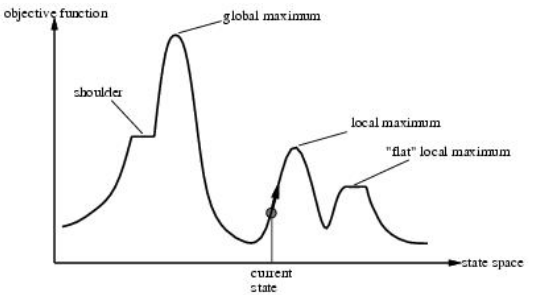
\includegraphics[width=7cm]{local.png}
    \caption{Objective function on the state space}
\end{figure}

\subsubsection{Neighbourhood}

\paragraph{Size} 
If we choose  to take larger neighbourhood we  will have \textit{shorter
path}  to the  solution, but  we will  also need  \textit{more time}  to
explore all possibilities. It's a \textbf{key design decision} (\textit{choice
between length of path and exploration})

\paragraph{Connectivity}

From each solution  there is a path  to an optimal solution.  It has two
advantages:
\begin{itemize}
    \item Required for convergence property
    \item No need of restarting strategy (you will never be block)
\end{itemize}

\paragraph{Constraint}

\textit{How to combine faisability with optimality requirements?} Two approaches are possible:
\begin{itemize}
\item
	\begin{enumerate}
	\item Maintain feasibility at all times
	\item Explore only feasible solutions
	\end{enumerate}
\item 
	\begin{enumerate}
	\item Do not maintain feasibility at all time; relax a subset of the constraints
	\item Explore a larger search space
	\item Drive the search to high quality and feasible solutions
	\end{enumerate}
\end{itemize}

\subsection{Heuristics and metaheuristics}

\begin{description}

    \item[Heuristics] focus on  chosing the next solution  and drive the
    search  towards \textit{local  optimum} based  on local  information
    (\textit{current solution and its  neighborhood}). It's a memoryless
    solution.

        \begin{itemize}
            \item Hill-climbing
            \end{itemize}

    \item[Metaheuristics] Try to escape from  local and drive the search
    towards  \textit{global optimality}  based on  collected information
    on  the   execution  sequences.  It  includes   memory  or  learning

        \begin{itemize}
            \item Iterated local search
            \item Simulated annealing
            \item Guided local search
            \item \ldots
            \end{itemize}

    \item[Systematic heuristics]  Exploration (possibly partial)  of the
neighborhood to determine the next solution

\end{description}

\subsection{Algorithm: Hill climbing}

Move on  the direction of increasing  value and stop the  iteration when
it's impossible to go further.

This algorithm go quickly to a best solution but he have multiple issues :
\begin{itemize}
    \item Local maximum 
    \item Plateau : \textit{a maximum flat area} can stop the algorithm
    \item Ridges : sequence of local maxima where Hill climbing are very difficult to navigate
\end{itemize}


Hill climbing depend  very  much on  the  shape  of  the state-space  landscape!  Hill
climbing has a  big Achilles hell, the local maximas.  You cannot escape
local maxima,  considering that  hill climbing \textbf{will  never makes
downhill moves}.

\subsubsection{Variants}

There is multiple variants of the hill climbing algorithm:
\begin{description}
    \item[Stochastic hill climbing] randomly choose in the list of uphill moves
    \item[First-choice hill climbing] pick the first good successor you find 
        (\textit{useful when there is a large amount of possibilites})
    \item[Random restart] You start from multiple random points
\end{description}


\subsection{Random walks}

You can consider another kind of heuristic, in which you select randomly
an  element of  the  neighborhood and  decide whether  to  accept it  as
the  next solution.  There  is two  possibles approches:  \textit{random
improvement}  and  \textit{metropolis heuristic}  \textbf{TODO  Complete
with the book}.


\subsection{Simulated annealing}
Combine RW and HW to make a complete and efficient algorithm.
The algorithm start by randomize hard and then gradually reduce the intensity of randomized
and take more the best solution in neighboor.

(\textit{Annealing is the process of heating metal and letting it cool slowly to lock in the stable locations of the molecules} )

So here is the principle of this technique:
\begin{enumerate}
	\item Always move uphill if possible (hill climbing)
	\item Sometimes go downhill (like in metallurgy when temperature is high).
	\item Optimality is guaranteed with slow annealing schedule. 
\end{enumerate}


\subsection{Local beam search}

Hill climbing and simulated annealing techniques keep one state in memory. 
In this technique you keep $k$ states in memory and at each step all state 
generate successors and we take the $k$ best one.

(\textit{Information between state can be shared, like
``Come over here, the grass is greener''}).
In pratcice, local beam search suffer from a lack of diversity because
state quickly become concentrated in a small region.


\paragraph{ } A stochastic beam search (like stochastic hill climbin)
help to alleviate this problem


\subsection{Genetic algorithms}  

Based on theory  of  evolution, start  whith  k initial  state.
(\textit{population})  and the  next  generation is  produce by  merging
between individuals from current population. 

A individual is represented by a fixed-length string and is \textit{fitness}
(score for each state, greater is better) is evaluated.

\paragraph{Cross over} A cross over point is choose at each reproduction. (it's the position where
the pair will be merged)
The goal is to can produce s state that is long way from either parent state.
( ex: avec cross over at point 3, AAACCCC andDDDEEEE $\to$ AAAEEEE and DDDCCC)


\paragraph{Random mutation } can also perfom for explore new parts of
search space, but do this with a low probability to no break a good solution!


\paragraph{ } 
Good compromise between go to the better, random exploration and shared information
between many state.
The only issues with this algorithm is that crossover is not applicable to all problems.

\subsection{Tabu search Metaheursitics}:
You select  the best  neighbor that  has not yet  been visited  and only
maintain a suffix of the sequence visited node, not all of them.

An abstraction is used to represent the suffix (to reduce the memory). We change the suffix
if the move improve the best solution so far.

\subsection{Intensification vs Diversification}
\begin{tabular}{m{8cm}|m{8cm}}
Intensification & Diversification \\
\hline

	\begin{description}
		\item[Goal] increase search around promising areas
		\item[Risk] premature convergence
		\item[Mean] favor good solutions
	\end{description}
&
	\begin{description}
		\item[Goal] explore new ares
		\item[Risk] convergence to optimality may be too long
		\item[Mean] probabilistic choice of solutions
	\end{description}
\end{tabular}

\subsection{Other local search Approaches}

There is a bunch of other local search:
\begin{description}
    \item[Variable Neighborhood Search] sequence of neighborhood
    \item[Guided local search] use a sequence of objective functions to drive away from local optima
    \item[Adaptive local Search] The heuristics/metaheuristisc are dynamically adapted during the search
    \item[Ant colony optimization] the selection function is updated
    \item[Statistic Local Search] another name for Local search, stressing the stochastic aspect of the search
\end{description}



\section{Chapitre 5 : Adversial search}

\subsection{Game}

\textbf{Game theory} view any multiagent environment as a game, provided that
the impact of each agent on the other is \textit{significant}.

In ia the most common games are deterministic (\textit{fully observable with utility value at
the end of the game are always equal en opposite}), turn-taking, two-player, zero-sum game of
perfect information (if someone win, the other loose).

There is also game with imperfect information and not deterministic value because of chance.


\textbf{A game} :
\begin{description}
    \item[Initial state] ($s_0$) and who is playing first.
    \item[Player (s)] : which player has move
    \item[Actions (s)] : set of legal move
    \item[Result (s, a)] : \textit{transition model} which define result of a move
    \item[Terminal set (s)] 
    \item[Utility (s,p)] : \textit{utility function} define the final numeric value for a game that ends in terminal state s for a player p.
        \textit{zero-sum game} defined as one where the total payoff to all players is the same for every instance of the game.
\end{description}

\textbf{Game tree} : tree where node are game state and edge are move.

\begin{figure}[h]
\centering
\begin{tabular}{|l|m{3cm}|m{3cm}|m{3cm}|m{3cm}|}
\hline
& \textbf{MinMax} & \textbf{Prunning} & \textbf{H-MinMax} & \textbf{ExpectMin} \\
\hline
& All tree & with alpha-beta & Limited depth & Stochastic \\

\hline
\hline
\textbf{Complete} & \textcolor{red}{if} \textbf{tree} finite & \textcolor{red}{if} \textbf{tree} finite  & YES  & YES \\
\hline
\textbf{Optimal} & YES & YES & NO & NO \\
\hline
\textbf{Time} & $b^{m}$    & $b^{d/2}\textrm{ or }b^{3d/4}$ & $b^l$ & $b^m n^m$\\
\hline
\textbf{Space} & $bm$ & $bd/2\textrm{ or }3bd/4$ & $bl$ & $b^m$ \\
\hline

\end{tabular}
\caption{Adversial Search Algorithm}
\end{figure}



\subsection{Optimal decision}
Given game tree, optimal strategy be determined from the minimax value of each
node.. \textit{assuming that both players play optimally}.

Minimax is perfect play for deterministic game and if the opponent don't play
optimally, he is better.

\begin{figure}[h]
    \centering
    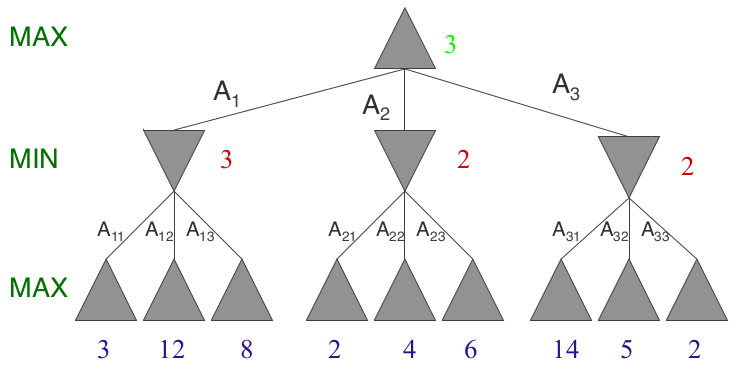
\includegraphics[width=10cm]{minmax.png}
    \caption{Minmax}
\end{figure}

\subsubsection{Algorithm: minmax}
Generate game tree to the terminal states and apply the utiliy function on these state.
After apply minmax to go on the top and value determine move.

Minmax is complete if tree is finite.

\paragraph{Complexity} 
Such as minmax perform a \textcolor{red}{DFS} on the game tree, the \textit{space} complexity is O($bm$) 
or O($m$) if action are genetare one at a time.

\textit{Time} complexity is O($b^m$).

\subsubsection{Optimal decisions in multiplayer games}
When there are more than 2 players, we keep and vector at each node , where element of the vector are the 
utility of each player. Each player will choose the move that maximize is utility function.

\subsection{Alpha-beta pruning}
\begin{figure}[h]
\begin{tabular}{m{10cm}m{6cm}}
    \centering
    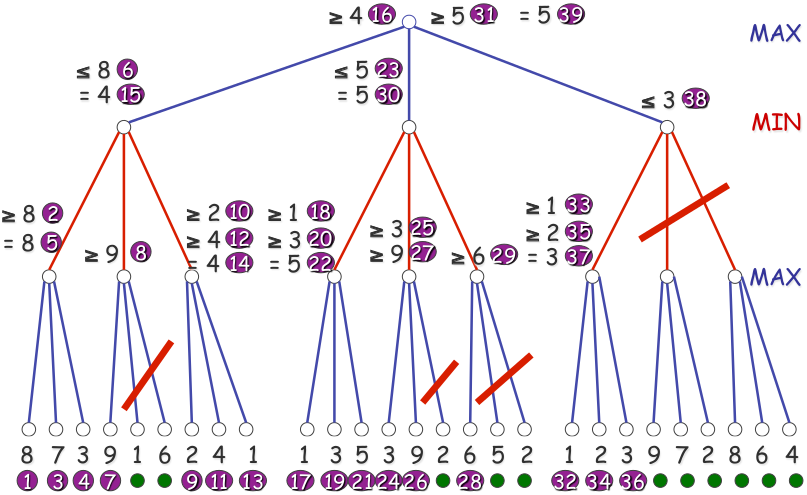
\includegraphics[width=10cm]{minmax_ex.png}
&

\begin{description}
    \item $\mathbf{\alpha}$ : value of the best (\textit{higher}) choice found
        so far at any choice point along the parth for \textbf{MAX}
    \item $\mathbf{\beta}$ : value of the best (\textit{lowest}) choice found
    so far at any choice point along the parth for \textbf{MIN}
\end{description}
\end{tabular}
\end{figure}

Pruning does not affect final result.

\paragraph{Complexity} if successors are ideally visited, \textit{time} complexity
is O($b^{(d/2)}$) and if visited randomly O($b^{3d/4}$)


\subsubsection{Move ordering}

Alpha beta prunning is highly dependent on the order in which the states are examined.

\paragraph{ }\textbf{Killer move} are the best move. If they visitited first in a Alpha-beta pruning algorithm,
the algorithm will perform more efficiently.


\paragraph{Game graph} There are repeated states in many games because of \textbf{transpositions}.
To be efficient, we can store the evaluation of state in hash table called \textbf{transposition
table}.

This table can doubling the reachable search depth in chess, but whith a million node per second,
it's no possible to keep all node in table\ldots To solve this, various strategie
choose wich node to keep and wich to discard.

\subsection{Imperfect real-time decisions}
In practice, make complete game tree is usually not pratical.
So, program should cut off the search earlier and apply a heuristic \textbf{evaluation
function} on states in search to estimate the expected utility.

Change minmax :
\begin{enumerate}
    \item Utility function by heuristic evaluation function (\textsc{eval})
    \item Replace terminal set by a cuttoff test that decide when apply \textsc{eval}
\end{enumerate}

\subsubsection{Evaluation function}
\begin{itemize}
    \item Must be consistent with the utility function.
    \item Tradeoff between accuracy and time cost.
    \item Reflect the actual chances of winning.
    \item Weighted \textbf{linear function} are frequently used with a combination of features.
\end{itemize}

We used weighted linear function only if the feature are independent (For exemple some piece in the chess
are more powerful at the end of the game because there is more space). So some program use non linear 
combinations of feature. 


\subsubsection{Cutting off search}
The most straightforward approach ti to set a fixed depth limit.
But there is a issue if the state is favorable to fast change in the next
state\ldots 

\paragraph{Quiescent}  To solve  this problem,  the evaluation  function
should  be applied  only to  position that  are \textbf{quiescent},  i.e
stable state. (\textit{unlikely  to exhibit wild swings in  value in the
near futur})

\paragraph{Horizon effect} We can delay disasters, but we don't prevent them. It could happens because of
cut-off as the horizon is not deep enough.

\subsubsection{Forward pruning}
Some moves at a given node are pruned immediatly without further consideration.
Is cutoff moves you know are bad.

\paragraph{ } One approach is \textbf{beam search} : considere onlyt a ``beam'' of the 
\textit{n} best moves rather than all possible moves.


\subsubsection{Search vs Lookup}
For many game, table lookup are used for the opening and end of the game. Because at first (at the end) the 
situation are very similar. After some moves, the actual search must be done because situation differs. 



\subsection{Stochastic games}
Is a game with a dregree of unpredictability through random elements.

$\rightarrow$ Requires chance nodes in addition to the max/min nodes

\textbf{Exapectminimax} algorithm is this one.

\paragraph{Complexity} \textit{time} complexity is O($b^m n^m$) where $n$
is the number of distinct chance events and \textit{space} complexity is O($b^m$)

\begin{figure}[h]
    \centering
    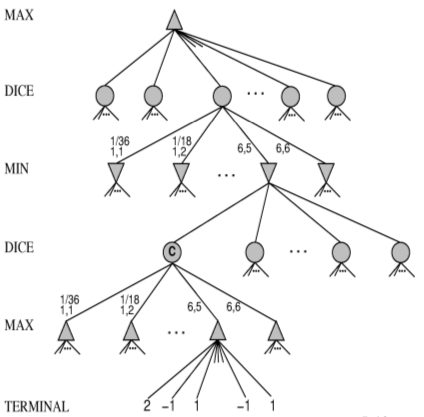
\includegraphics[width=5cm]{stochastic.png}
    \caption{Game with dice node}
\end{figure}


\subsubsection{Evaluation  function for  game  of  chance} 

The  evaluate function  can  be  totally differentyl  if  we change  the
random event.  So, the \textbf{evaluation  function} must be  a positive
linear transformation  of the  probability of  winning from  a position.
(\textit{more generally of the expected utility of the position})

\paragraph{Alternative :} Monte carlo simulation
consist of using the alpha beta pruning. Then at a node,  play against itself a thousand game using random 
dice rolls. The win percentage is a good approximation of the value of function. 



\subsection{Partially observable games}
TODO %Je crois pas que c'est utile

\subsection{State-of-the-art Game programs}
TODO%pareil


\section{Chapitre 6 : Constraint Satisfaction Problem }

\subsection{Defining CSP}
	A CSP consists of three components X,D and C:
	\begin{itemize}
		\item X is a set of variable,${X_1,...,X_n}$.
		\item D is a set of domains${D_1,...,D_2}$, one for each variable.
		\item C is a set of constraint that specify allowable combinations of values
	\end{itemize}

 Element of  C consits  of a pair  <scope,rel>, where  \textit{scope} is
 tuple of all the variables involved and \textit{rel} is their relation.

 \paragraph{Assigment} It represents the state  of an CSP and where each
variable have a value in its domain.

 \paragraph{Solution} in a CSP is a consistent assignment (an assignment
 that does not violate any constraint)

 \paragraph{Constraint  graph}  is  a  graph where  the  nodes  are  the
variable and the arc are the constraint

	There is different type of CSP , depending on the domain:
	\begin{itemize}
		\item Discrete and finite domains (ex: Combinatorial problems).
		\item Discrete and infinite domains (ex:Scheduling).
		\item Continous (and infinite) domains.
	\end{itemize}
	And types of constraints:
	\begin{itemize}
		\item unary constraints : on only one variable (ex: x $\neq$ green)
		\item binary constraints : on two variable (ex: x+y $\leq$ 12)
		\item high-order constraints : over several variable (ex: x+5y-3z $\leq$ 8)
	\end{itemize}
	We only consider only CSP with binary constraints.

 \paragraph{Hypergraph}   An   hypergraph   is   graph   with   ordinary
 nodes (circle)  which   are  the   variable  and  the   constraint,  and
 hypernode (square) which represent the n-ary constraint.

\subsection{Constraint Propagation}

The objective  is to reduce the  search space. To achieve  that, we will
try to find  an equivalent CSP to the original  one with smaller domains
of variables.

There are to techinque to reduce the size of the domain when considering
constraint \textbf{locally}:
\begin{itemize}
    \item  Arc  consistency  consider  constraint  between  two  variables
      (remove uncompatible value in domain)
    \item Path consistency consider constraint between n variables.
\end{itemize}

\paragraph{Node consistent} All  the value in a  variable domain satisfy
the variable unary constraint

\paragraph{Arc consistent} All the value  in variable domain satisfy the
binary constraint

\paragraph{Path   consistent}   A   two-variable  set   ${X_i,X_j}$   is
path  consistent  with  respect  to  a  third  variable  $X_m$  if,  for
every  assignment  ${X_i=a,X_j=b}$  consistent with  the  constraint  on
${X_i,X_j}$,  there  is  an  assignement to  $X_m$  that  satisfies  the
constraints on ${X_i,X_m}\quad{X_m,X_j}$


TODO bound consitency

\paragraph{Global constraint}  Constraint involving an  arbitrary number
of variable and ad hoc specialized method (ex: Alldiff(X1,X2,..,X8))


\subsection{Backtracking Search for CSPs}

\subsubsection{Incremental formulation of CSP search }
\begin{itemize}
	\item The initial state is an empty assignment
	\item The succesor function assign a value to an unassigned variable provided no constraint violated
	\item The goal test check if the assignment is consistent and complete
	\item There is a constant value per step. (Path is irrelevant)
\end{itemize}

    
\paragraph{Commutativity} order the of application  of any given set of
action has no effect on the outcome.  

The \textbf{search tree} have a depth  of n (number of variable) and the
number of  state =  $O(d^n)$ with  d the  size of  the domain.  

Because there is $d$ value for $n$  variable we can expect a search tree
with $n! d^n$  \footnote{Branching factor on the top is  nd, at the next
level (n-1)d,\ldots} leaves with only $d^n$ possible assignement.

\paragraph{\textbf{But}} with CSP search algorithms should only consider
a single variable at each  node because with \textbf{commutativity} when
assigning values  to variables,  we reach  the same  partial assignement
regardless of order. 


\subsubsection{Backtracking search}  It's a  depth first search  that choose
values for one variable at a time  and backtracks when a variable has no
legal values left  to assign. 

When  choosing variable  in order,  it's  not efficient.  To reduce  the
search,  we  will improve  the  way  we  choose  the variable.  This  is
\textbf{variable ordering}.

\subsubsection{Variable ordering}
It exists two kind:
\begin{itemize}
    \item \textsc{Minimum Remaining Value}: we choose the variable with the fewest legal values. (first-fail heuristics)
    \item \textsc{Degree Heuristic}: Choose the variable involved in the largest number of constraints (it reduce the branching factor)
\end{itemize}

\subsubsection{Interleaving search and inference} 
When we make choice of a value for a variable, we have a brand-new opportunity to infer new
domain reductions on the neighboring variables.

To \textbf{reduce the search  space} and be more efficient in  the search, a good
idea is to progate the information to other constraints. 

It  is  done  with  \textit{Forward  checking,  consistency  and  global
constraint}.

\paragraph{\textbf{Forward checking} }
When X is assigned a value v:
\begin{itemize}
	\item Look at each unassigned variable T connected to X (with binary constraint).
	\item Remove from Y's domain the value inconsistent with the valuer chosen for X.
	\item With MRV, failure occurs if a domain becomes empty.
\end{itemize}

\subsubsection{Intelligent Backtracking}  Instead of  backing up  to the
preceeding variable, we back up to  a variable an try another value that
might fix the problem.

To achieve that we keep a \textbf{conflict set} for each value that keep
the assignement that are in conflict with this value.

With \textbf{backjumping} we go to  the most recent variable in conflict
set.

\paragraph{Conflict-directed backjumping} TODO


\subsection{Local Search for CSP}

\subsubsection{Complete state formulation of CSP search }
\begin{itemize}
	\item The initial state have a value to every variable
	\item The succesor function change a value of one variable
	\item The goal test check if the assignment is consistent and complete
	\item There is a constant value per step. (Path is irrelevant)
\end{itemize}

\paragraph{Min-Conflict} We choose the value with the minimum number of conflicts.

\subsection{Structure of the problem}

\subsubsection{Independent subproblem}

We   divide    the   the   CSP   in    \textbf{independent   subproblem}
(\textit{partition of  variable and constraint}) to  forming k different
CSP.

We can solved them separately and the solution is the union of the different
solution. The \textit{time complexity} is reduce to $O(d^{n/k} k)$

To achieve that, we consider  the \textbf{connected component} of
the constraint graph as a subproblem.

\subsubsection{Tree-structure subproblems}

\begin{description}
    \item[Directed arc consistency] under an ordering of variables $X_1, X_2, \cdots, X_n$
        IF every $X_i$ is arc-consistent with each $X_j$ for $j > i$
    \item[Topological sort] : Ordering of variable such thtat each variable 
        appears after its parents in the tree
\end{description}

Tree-structure  can be  solve in  \textit{time complexity}  of $\color{red} O(nd^2)$
because  any tree  with  $n$ node  has  $n-1$  arcs and  we  can make  a
\textbf{directed arc-consistent} in  O($n$) step where we  need to check
the arc-consistent in $O(d^2)$.


\paragraph{Removing nodes}
\begin{enumerate}
    \item Choose a cycle subset S (size c)
    \item For each possible \textbf{assignement} to the variables \textbf{S} that satisfies all constaint on S
        \begin{enumerate}
            \item \textbf{Remove} in domain any variables that are inconsistent with the assignement of S
            \item If CSP has solution, return it with S assignement
\end{enumerate}

\subparagraph{ } Finding the smallest cutset is NP-hard


\paragraph{Grouping nodes}
\begin{itemize}
    \item Each variable appears in at least one subproblems
    \item Two variable connected by a constraint must appear together
        in at least one subproblem
    \item TODO

\subparagraph{ } Finding decomposition with minimal tree is NP-hard


\section{Chapitre 7 : Logical agent}
Achieving a goal frequently requires more than searching : \textit{planning,
reasoning and acting}.

\textit{In which we design agents that can form representations of a complex world, use a process of inference to derive new representations about the world and use these new representation to deduce what to do}

\subsection{Knowledge-based agents}

\textbf{knowledge-based agents} can reasoning with knowledge.

\begin{description}
    \item[Knwoledge base] : central component of KBA, this is a set of \textbf{sentence}
    \item[Background knowledge] : initialy knowledge of KB
    \item[Sentence] : assertions about the world
    \item[Axiom] : A sentence without being derived from other sentences (\textit{independant})
\end{description}

\paragraph{Opération on KBA} :
\begin{enumerate}
    \item \textsc{Tell} : add new sentence
    \item \textsc{Ask} : query what is know

    \item \textsc{Make-percept-Sentence} : construct a sentence asserting that the agent perceived
        the given percept at the given time.
    \item \textsc{Make-Action-Query} : construct a sentence that asks what action should be done at the current time
    \item \textsc{Make-Action-Sentence} : constructs a sentence asserting that the chosen action was excecuted
\end{enumerate}

There operations involve \textbf{inference} (deriving new sentences from old)

\paragraph{Called agent} is perform in three time :
\begin{enumerate}
    \item Tell the knowledge of KB
    \item What action should perform
    \item Tell wich action was choose and agend execute
\end{enumerate}

\paragraph{Knowledge level} :
TODO

\paragraph{Knowledge representation} :
TODO


\subsection{The Wumpus World}

\begin{itemize}
    \item Not fully observable (only local perception)
    \item Deterministic (outcome exactly specified)
    \item No episodic  (Sequential at the level of actions)
    \item Static (Wumpus and pits do not move)
    \item Discrete
    \item Single-agent (Wumpus is essentially a natural feature)
\end{itemize}

\paragraph{ } See page 209-210-211 of the book

\paragraph{ } Knowledge gained in different places at different times must
be combined to draw conclusions


\subsection{Logic}
\begin{description}
    \item[Syntax] : Specifie all the sentences that are well formed
    \item[Semantic] : Define the \textit{truth} of sentences respect to each
        possible world (interpretation)
    \item[Interpretation] : mathematical abstraction of a possible world
    \item[Model of sentence $\alpha$] is an interpretation where the sentence 
        is true. 
    \item[M($\alpha$)] : set of all model of $\alpha$
\end{description}

\subsubsection{Entailment} 
$$\textrm{Entailment between } \alpha \textrm{ and } \beta
\quad \equiv \quad \alpha \models \beta  \quad IFF \quad M(\alpha) \subset M(\beta)$$
$\beta$ is true in every model of $\alpha$ (example $x=0 \models xy=0$)

\begin{figure}[h]
    \centering
    \begin{tabular}{cc}
        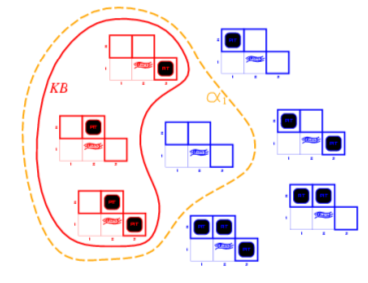
\includegraphics[width=6cm]{alpha_1.png}
        &
        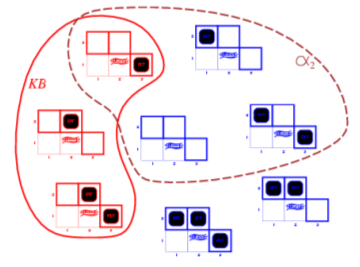
\includegraphics[width=6cm]{alpha_2.png}
        \\
        $\alpha_1$ = ``No pit in 1,2''
        &
        $\alpha_2$ = ``No pit in 2,2''
        \\
    \end{tabular}
    \caption{Wumpus models conclusion}
\end{figure}

If $KB \models \alpha_1$ we can conclue that $\alpha_1$ is true!


\paragraph{To verifu $KB \models \alpha$} use \textbf{model checking}.\\
\begin{tabular}{m{11cm}m{1cm}m{1.5cm}m{1cm}}
    \begin{itemize}
        \item enumeration of the interpretations
        \item Find the interpretations wich are models of $\alpha$
        \item Chech that $\beta$ is these models $\color{red} \alpha \vdash \beta$
    \end{itemize}
    &
    \textcolor{red}{Completeness}
    &
    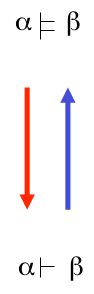
\includegraphics[width=1cm]{soundness.png}
    &
    \textcolor{blue}{Soundness}
    \\
\end{tabular}


\subsection{Propositional Logic}

\subsubsection{Syntax}
$\neg$,
$\wedge$,
$\vee$, 
$\Rightarrow$, 
$\Leftrightarrow$.

\subsubsection{Semantic}
With \textit{thuth table}

\begin{figure}[h]
    \centering
    \begin{tabular}{|c|c||c|c|c|c|c|}
        \hline
        P & Q & $\neg P$ & $P \wedge Q$ & $P \vee Q$ & $P \Rightarrow Q$ & $P \Leftrightarrow$ \\
        \hline
        F & F & T & F & F & T & T \\
        F & T & T & F & F & T & F \\
        T & F & F & F & F & F & F \\
        T & T & F & T & T & T & T \\
        \hline
    \end{tabular}
    \caption{Truth table}
\end{figure}


\subsubsection{Simple inference}
Goal is to decide whether $KB \models \alpha$. 
\textbf{Model-checking approach} :
\begin{enumerate}
    \item Enumerate the interpretations ($2^n$ where $n$ is the number of symbol)
    \item Check wheter $\alpha$ = $P_{1,2}$ is true in every model of KB
\end{enumerate}

The algorithm is \textit{sound} because it impletments directly the definition of entailment and \textit{complete} because it work for any $KB$ and $\alpha$.

\paragraph{Complexity} \textit{time} complexity is O($2^n$) and \textit{space} complexity
O($n$) because it's a \textcolor{red}{depth-first}.


\paragraph{} Note that propositionnal entailment is co-NP-complete so every know inference
algorithm for propositionnal logic has a worst-case complexity that is exponential in
the size of the input.

\subsection{Propositional Theorem Proving}

\begin{description}
    \item[Logical equivalence] : $\alpha \equiv \beta$
    \item[Valid] : true in all interpretation
    \item[Satisfiable] : true in some interpretation
    \item[Unsatisfiable] : always false
    \item
    \item $\alpha \models \beta \quad IF \quad (\alpha \wedge \neg \beta)$ is unsatisfiable
\end{description}

\subsubsection{Inference proof}
See all inference on page 222-223

\paragraph{Search algorithm} can be use to find a sequence of steps that constitutes a proof.
We just need to define : 
\begin{itemize}
    \item \textsc{Initial State} : the initial knowledge base
    \item \textsc{Actions} : The set of action is all the inferences rules
    \item \textsc{Result} : The result of a action is to add the sentence in the bottome half of the inference rule
    \item \textsc{Goal} : Contains sentence we are trying to prove
\end{itemize}

\subparagraph{\textbf{Monotonicity}} is a property of logical systems.
$$ IF \quad KB \models \alpha \quad THEN \quad KB \vee \beta \models \alpha$$

This knowledge might  help the agent draw additionnal  conclusion but it
cannot invalidate any conclusion $\alpha$ already inferred.


\subsubsection{Proof by resolution}
The resolution inference rule need to be sound and complete and use with a 
complete search algorithm.

\paragraph{Conjunctive normal form} 
$$(l_{1,1} \vee \cdots \vee l_{1,k}) \wedge \cdots \wedge (l_{n,1} \vee \cdots \vee l_{n,l})$$

Every sentence of propositional logic is logically equivalent to a conjunction of clause using this step :
\begin{enumerate}
    \item Eliminate $\Leftrightarrow$
    \item Eliminate $\Rightarrow$
    \item Move $\neg$ inside
    \item Distribute $\wedge$ over $\vee$
\end{enumerate}

\paragraph{A resolution algorithm}
This algorithm proof by contradiction $(KB \vee \neg \alpha)$ because $$KB \models \alpha \quad
 IF \quad (KB \vee \neg \alpha)$$

TODO

\paragraph{Completeness of resolution}
Resolution is \textbf{completeness} because if a set of clauses is unsatisfiable, then
the resolution closure of those clauses contains the empty clause.


\subsubsection{Horn clauses an definite clause}
\begin{description}
    \item[Definite clause] : a disjunction of literals of wich exactly one is positive 
        ($\neg L_1 \vee \neg Breeze \vee B_{1,1}$)
    \item[Horn clause] : a disjunction of literals of wich at most one is positive
    \item[Goal clause ] : a disjunction of no positive literals
\end{description}

Knowledge base containing only \textbf{definite clause} for three reasons :
\begin{enumerate}
    \item Every finite clause $(\neg L_1 \vee \neg Breeze \vee B_{1,1})$ can be write as an 
        implication$(L_{1,1} \wedge Breeze) \Rightarrow B_{1,1}$
    \item Inference with Horn clauses can be done through the \textit{forward-chaining} and 
        \textit{backward-chaining}
    \item Decice \textbf{entailment} with horn clause can be done in time
        that is \textit{linear} with the size of KB
\end{enumerate}

\subsubsection{Forward and backward chaining}

\begin{figure}[h]
    \centering
    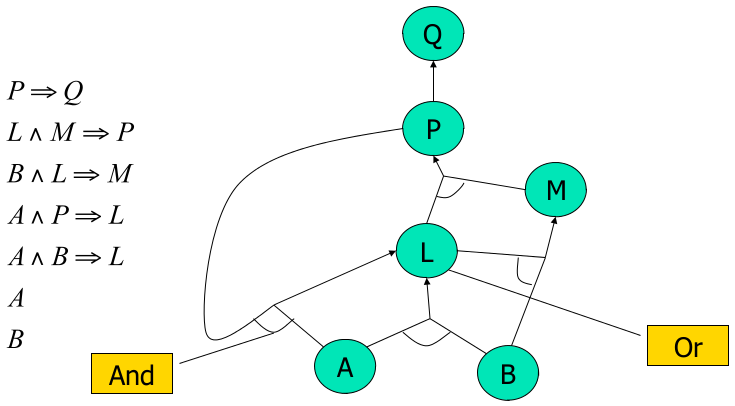
\includegraphics[width=10cm]{andor.png}
    \caption{A set of horn clause with the corresponding \textsc{and-or} graph}
\end{figure}


See the example on annexe.

\paragraph{Forward}
We start on the know leave (Here A and B). After we cross on the graph 
and when a \textit{literal}, q,  is reached then $KB \models q$.

It's easy to see that every definite clause in the original KB is true
for this model.

In conclusion, to prove $KB \models q$, a forward chaining is perform
with the KB and q. If q is reached then $KB \models q$

\paragraph{Backward}
It's the same idea but we start on sequence q to go-back.


\subsection{Effective Propositional Model Checking}
TODO

\subsubsection{Algorithm: Davis-Putman}

\subsubsection{Local search algorithm}

\subsubsection{Landscape of random SAT problem}

\subsection{Agent based on propositional logic}
TODO

\section{Chapitre 8 $\backslash$ 8.3.3 : First-Order logic }
\subsection{From Propositional logic to First-Order logic}
	Propositional logic lacks expressive power to describe the environment 
	concisely (ex: cannot say `pits 	cause breezes in adjacent squares'). 
	Then we use First-Order logic, it assumes the world contains:
	\begin{itemize}
		\item Object: people,houses,numbers,...
		\item Relation: unary, n-ary, inside,...
		\item Function: successors, father\_of,...
	\end{itemize}
\subsection{Syntax and semantics of FOL}
	TODO add BNF GRAMAMAR 
	The semantics is provided by interpretation for the basic constructs. The interpretation maps 
	constant, function symbols and predicat symbols to the domain.
	For closed well-formed formulas F (no non-quatified variable )
	\begin{itemize}
		\item $\forall x$ F(x) is true if $\forall d\in D$,I(F(d)) = true
		\item $\exists x$ F(x) is true if $\exists d\in D$,I(F(d)) = true
	\end{itemize}
	\paragraph{Model} An interpretation where a sentence $\alpha$ is true.
	\paragraph{Logical entailment} between sentence $\alpha \quad and \quad \beta$ $\alpha\models\beta$
	iff, $\beta$ is true in every time $\alpha$ is true.
	\paragraph{Validity} a sentence is true in all interpretations.
	\paragraph{Satisfiability} a sentence is true in some interpretations.
	\paragraph{Inconsistency/unsatisfiability} a sentence is false in all interpretation.
	With FOL we can use the quantifier($\forall,\exists$) to express properties of collections of objects.
	\begin{itemize}
		\item $\forall x\quad Human(x) \Rightarrow Mortal(x)$
		\item $\exists x \quad Bird(x) \wedge \neg Can-Fly(x)$
	\end{itemize}
	Take care the order of the quantifiers is important.  We can express complex sentences with multiple 
	variables and by nesting quatifiers(using several variable instead of several same quantifier).
	
	The connection between the two quantifier is defined as follow:
	\begin{itemize}
		\item $\forall\quad \neg P(x) \equiv \neg\exists x \quad P(x) $
		\item $\forall\quad P(x) \equiv \neg\exists x \quad \neg P(x)$
	\end{itemize}
\subsection{Using FOL}
	Sentences are added in the KB  with \textit{TELL} (ex: Tell(KB,King(John))). Queries are made to the 	
	KB with \textit{ASK} (ex: Ask(KB,King(John))), it will return a list of variable/term pairs that
	satisfies the query.
	\paragraph{Family Relationships} It's a domains that contains fact of familial relation.
\subsection{Knowledge Engineering}
\section{Chapitre 9 : }
TODO

\section{Chapitre 10 : }
TODO

\section{Chapitre 11 $\backslash$ 11.2, 11.4 : }
TODO

\section{Chapitre 18.1-3, 18.10 : }
TODO


\section{Annexe}
%\includepdf{forward_example.pdf}

\begin{thebibliography}{1}
\bibitem{wikiadmheur} http://en.wikipedia.org/wiki/Admissible\_heuristic, {\em Wikipedia}
%\bibitem{Propagation} P.G. Fontolliet, {\em Traité d'Electricité}, Volume XVIII, Ecole polytechnique fédéral de Lausanne, pp 72-73
\end{thebibliography}

\end{document}
